% DPF 09 talk on strangeness in nucleon

\documentclass[10pt]{beamer}
\usefonttheme{professionalfonts} % using non standard fonts for beamer
\usefonttheme{serif} % default family is serif
\usepackage{amsmath}
\usepackage{mathtools}
%\documentclass[12pt]{beamerthemeSam.sty}
\usepackage{epsf}
%\usepackage{pstricks}
%\usepackage[orientation=portrait,size=A4]{beamerposter}
\geometry{paperwidth=160mm,paperheight=120mm}
%DT favorite definitions
\def\LL{\left\langle}	% left angle bracket
\def\RR{\right\rangle}	% right angle bracket
\def\LP{\left(}		% left parenthesis
\def\RP{\right)}	% right parenthesis
\def\LB{\left\{}	% left curly bracket
\def\RB{\right\}}	% right curly bracket
\def\PAR#1#2{ {{\partial #1}\over{\partial #2}} }
\def\PARTWO#1#2{ {{\partial^2 #1}\over{\partial #2}^2} }
\def\PARTWOMIX#1#2#3{ {{\partial^2 #1}\over{\partial #2 \partial #3}} }

\def\rightpartial{{\overrightarrow\partial}}
\def\leftpartial{{\overleftarrow\partial}}
\def\diffpartial{\buildrel\leftrightarrow\over\partial}

\def\BI{\begin{itemize}}
\def\EI{\end{itemize}}
\def\BE{\begin{displaymath}}
\def\EE{\end{displaymath}}
\def\BEA{\begin{eqnarray*}}
\def\EEA{\end{eqnarray*}}
\def\BNEA{\begin{eqnarray}}
\def\ENEA{\end{eqnarray}}
\def\EL{\nonumber\\}


\newcommand{\map}[1]{\frame{\frametitle{\textbf{Course map}}
\centerline{\includegraphics[height=0.86\paperheight]{../../map/#1.png}}}}
\newcommand{\wmap}[1]{\frame{\frametitle{\textbf{Course map}}
\centerline{\includegraphics[width=0.96\paperwidth]{../../map/#1.png}}}}

\newcommand{\etal}{{\it et al.}}
\newcommand{\gbeta}{6/g^2}
\newcommand{\la}[1]{\label{#1}}
\newcommand{\ie}{{\em i.e.\ }}
\newcommand{\eg}{{\em e.\,g.\ }}
\newcommand{\cf}{cf.\ }
\newcommand{\etc}{etc.\ }
\newcommand{\atantwo}{{\rm atan2}}
\newcommand{\Tr}{{\rm Tr}}
\newcommand{\dt}{\Delta t}
\newcommand{\op}{{\cal O}}
\newcommand{\msbar}{{\overline{\rm MS}}}
\def\chpt{\raise0.4ex\hbox{$\chi$}PT}
\def\schpt{S\raise0.4ex\hbox{$\chi$}PT}
\def\MeV{{\rm Me\!V}}
\def\GeV{{\rm Ge\!V}}

%AB: my color definitions
%\definecolor{mygarnet}{rgb}{0.445,0.184,0.215}
%\definecolor{mygold}{rgb}{0.848,0.848,0.098}
%\definecolor{myg2g}{rgb}{0.647,0.316,0.157}
\definecolor{abtitlecolor}{rgb}{0.0,0.255,0.494}
\definecolor{absecondarycolor}{rgb}{0.0,0.416,0.804}
\definecolor{abprimarycolor}{rgb}{1.0,0.686,0.0}
\definecolor{Red}           {cmyk}{0,1,1,0}
\definecolor{Grey}           {cmyk}{.7,.7,.7,0}
\definecolor{Lg}           {cmyk}{.4,.4,.4,0}
\definecolor{Blue}          {cmyk}{1,1,0,0}
\definecolor{Green}         {cmyk}{1,0,1,0}
\definecolor{Brown}         {cmyk}{0,0.81,1,0.60}
\definecolor{Black}         {cmyk}{0,0,0,1}

\usetheme{Madrid}


%AB: redefinition of beamer colors
%\setbeamercolor{palette tertiary}{fg=white,bg=mygarnet}
%\setbeamercolor{palette secondary}{fg=white,bg=myg2g}
%\setbeamercolor{palette primary}{fg=black,bg=mygold}
\setbeamercolor{title}{fg=abtitlecolor}
\setbeamercolor{frametitle}{fg=abtitlecolor}
\setbeamercolor{palette tertiary}{fg=white,bg=abtitlecolor}
\setbeamercolor{palette secondary}{fg=white,bg=absecondarycolor}
\setbeamercolor{palette primary}{fg=black,bg=abprimarycolor}
\setbeamercolor{structure}{fg=abtitlecolor}

\setbeamerfont{section in toc}{series=\bfseries}

%AB: remove navigation icons
\beamertemplatenavigationsymbolsempty
\title{
  \textbf {Waves}\\
%\centerline{}
%\centering
%\vspace{-0.0in}
%\includegraphics[width=0.3\textwidth]{propvalues_0093.pdf}
%\vspace{-0.3in}\\
%\label{intrograph}
}

\author[W. Freeman] {Physics 211\\Syracuse University, Physics 211 Spring 2015\\Walter Freeman}

\date{\today}

\begin{document}

\frame{\titlepage}

\frame{\frametitle{\textbf{Announcements}}
  \Large
\BI
\item{First thing while it's still fresh: a recap of a problem from Exam 3}
\EI
}

\frame{\frametitle{\textbf{The static equilibrium problem}}

A 4m-long pole of mass 80 kg extends from the side of a building, angled at 60 degrees above the horizontal. One meter from the end of the pole, a sign of mass 50 kg is attached. To support the pole,
a horizontal cable runs from the end of the pole to the building. (See the attached figure.)


\bigskip
\bigskip
\bigskip
\bigskip

\centerline{  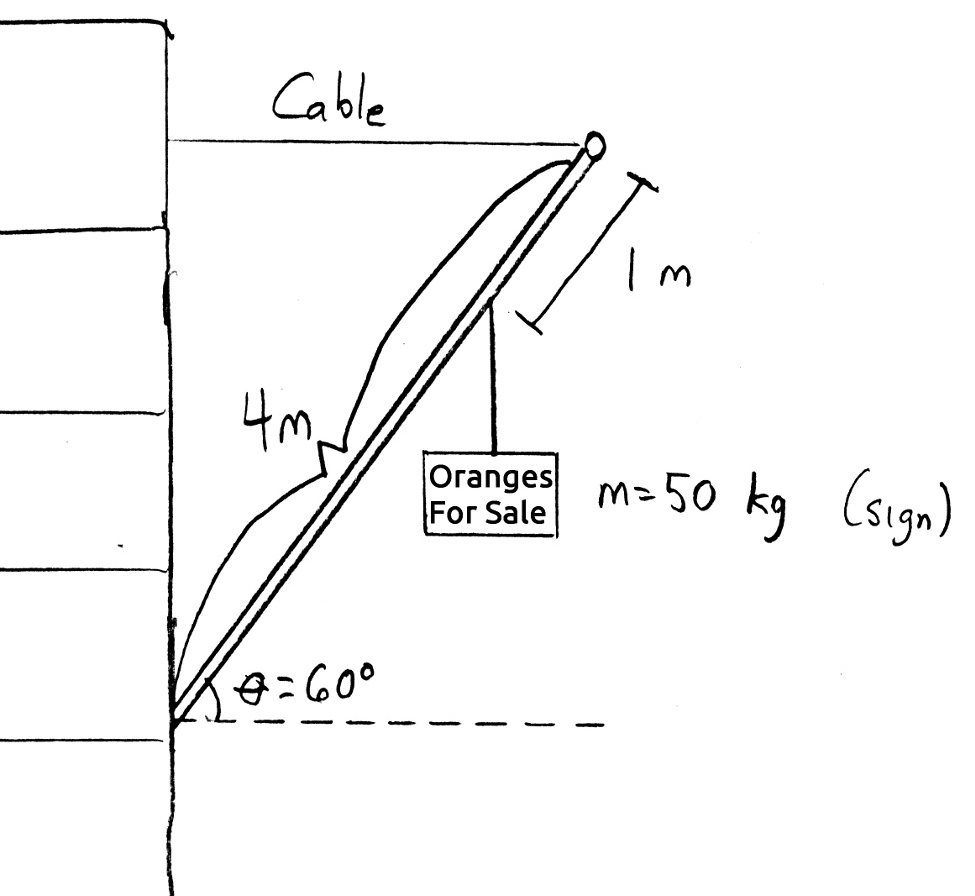
\includegraphics[width=0.4\textwidth]{sign2.jpg}}

\bigskip
\bigskip

... b) Compute the tension in the cable. (15 points)

}


\frame{\frametitle{\textbf{Grading and preparation for the final}}
    \large
  \BI
\item{Exam 3 will be graded out of 100}
\item{The average was around 55, which is not unusual for this exam}
\item{Full statistics available next week}
\pause
\item{Remember, you can drop one of your exam grades}
  \pause
\item{The final will be cumulative}
\item{More, easier problems; more conceptual problems}
\item{Multiple topical extra review sessions during the run-up to the final}
\item{Remaining recitation sections are {\bf all} review}
  \EI
}

\frame{\frametitle{\textbf{Final exam ``makeup opportunity''}}
  \Large
  \BI
\item{If you do substantially better on the final than one of your other exams...}
  \BI
\item{That exam counts less}
\item{The final counts more}
\item{This is being done {\bf after the curve}, so it can only help you}
  \EI
\EI
}

\frame{\frametitle{\textbf{Grade appeals for Exam 3}}
  \Large
  \BI
\item{To appeal your grade, you must attend Friday's recitation, and submit a correct solution with your appeal form}
  \BI
\item{(Remember recitation attendance counts toward your grade anyway!)}
  \EI
\item{Same procedure as before}
 \EI
 }



\frame{\frametitle{\textbf{Waves, overview}}
  \large
  \BI
\item{The next few classes are going to focus on the physics of waves}
\item{We'll use strings and tubes -- musical instruments -- as examples}
\item{... but all waves behave the same!}
  \BI
\item{Light waves}
\item{Radio waves: an antenna is just like waves on a string!}
\item{Sound waves}
\item{Water waves}
  \pause
\item{Matter waves in quantum mechanics: $s, p, d, f$ orbitals!}
  \EI
  \EI
}

\frame{\frametitle{\textbf{Waves in 1D -- modeling}}
  \BI
\item{Start with something empirical: can we model a vibrating string based on what we know so far?}
\item{Hooke's law describes elasticity, right?}
\item{Connect some Hooke's law springs between two points (simple3.c)}
  \pause
\item{This isn't very flexible, is it? How do we do better?}
  \pause
\item{Use more springs and masses (simple10.c)}
  \pause
\item{If we use very many of them, we should get ``real'' behavior}
  \BI
\item{Like pixels on a digital display: enough and you forget that they're there!}
\item{Now, what can we learn from how this behaves?}
\EI
\EI
}

\frame{\frametitle{\textbf{Waves in 1D -- learning from our model}}
  Some important properties: (pulse.c)
  \BI
\item{Pulses (regardless of their size or shape) go at a constant speed}
\item{{\bf The wave speed $c$} refers to how fast pulses travel down the string}
\item{The property of {\bf linearity:} (twopulse.c)}
  \BI
\item{Multiple pulses can pass through each other without interference}
\item{We will take this as absolutely true for our study here}
\item{Often not quite true for real waves -- very interesting behavior!}
  \EI
\item{Does a real string do this?}
  \BI
  \pause
\item{Wave speed $c$ goes up with more tension!}
  \EI
  \EI
}

\frame{\frametitle{\textbf{Sine waves}}
  \BI
\item{We're particularly concerned with waves that look like sines and cosines (sines.c)}
\item{These waves have two new properties: {\bf wavelength $\lambda$} and {\bf frequency $f$}}
\BI
\item{Wavelength: distance from crest to crest}
\item{Frequency: how many crests go by per second, equal to $1/T$ ($T$ = period)}
  \pause
\item{Speed = distance $\times$ time}
\EI
\EI
\Large
  $$c=\lambda f$$
  \BI
\pause
\item{What kind of sine and cosine waves can we put on our string?}
\item{Not any wavelengths will do, since the ends have to be fixed}
  \EI
}

\frame{\frametitle{\textbf{Standing waves}}
  \large
  \BI
\item{We can make a table of the wavelengths that will ``fit''}
  \pause
\item{$\lambda = 2L, 2L/2, 2L/3, 2L/4...$}
\item{$f = \frac{c}{2L}, 2\frac{c}{2L}, 3\frac{c}{2L}, 4\frac{c}{2L}...$}
\item{This is a remarkable result!}
  \BI
\item{Only certain frequencies of waves can ``live'' on my string}
\item{These are called ``standing waves''}
\item{This idea will occupy us for the rest of the course; for now, let's play! (harm.c)}
  \EI
  \EI
}




\end{document}
